\chapter{Guia de Referencia}

El presente capitulo no pretende ser un completo manual de usuario de la aplicacion, 
el sistema en si es bastante intuitivo en cuanto a su funcionamiento igual aqui
se resumira un poco el funcionamiento y algunas de las diferentes sessiones de de 
la Aplicacion.

\section{Organizacion de la Aplicacion}

La aplicacion se organiza de la siguiente manera, con las diferentes sessiones
bien definidas:

\begin{itemize}
    \item 1 Menu Principal
    \item 2 Menu Secundario
    \item 3 Cuerpo de la Aplicacion
    \item 4 Informacion de Usuario
\end{itemize}

\begin{figure}[H]
    \centering
    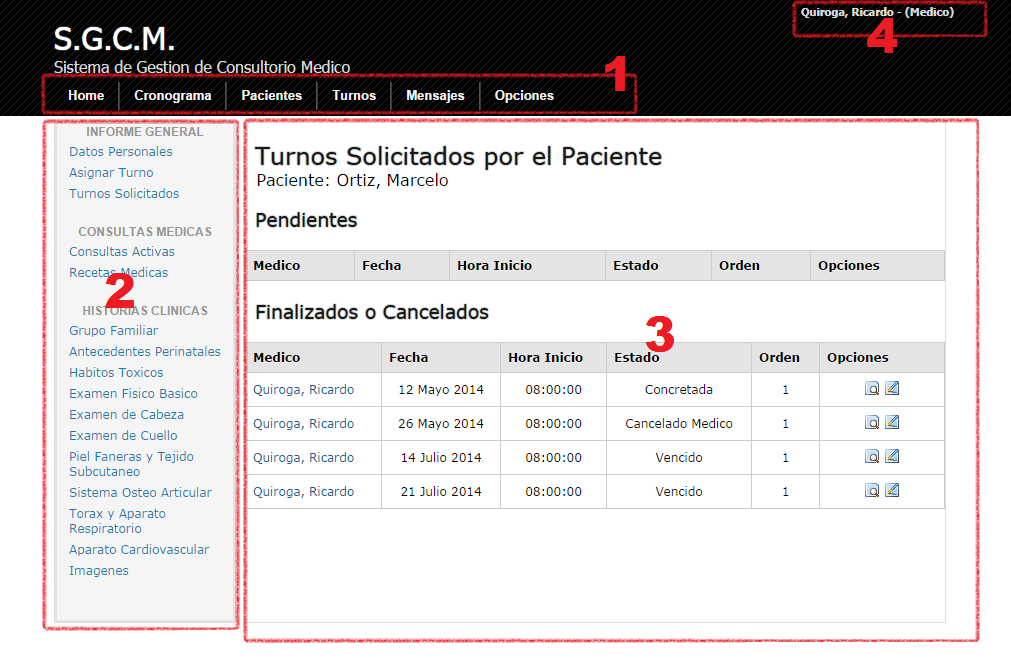
\includegraphics[scale=0.5]{resourse/organizacion.png}
    \caption{Organizacion Espacial del contenido de la aplicacion}
    \label{fig:61}
\end{figure}


\subsection{Menu Principal}

El contenido del menu principal depende del tipo de usuario que haya iniciado session
en base a ello tendra o no habilitadas diferentes funcionalidades de la aplicacion,
los unico menus comuneos son \textbf{Mensajes} y \textbf{Opciones}.


\subsection{Menu Secundario}

El menu secundario dependiendo de la vista donde se este, puede o no existir, y
su contenido dependera del las acciones que pueden ser realizadas en ella.


\subsection{Cuerpo de la Aplicacion}

Aqui se localizara el contenido principal de la vista, ya sea un formulario para
registrar alguna informacion, una lista para mostrar informacion etc.


\subsection{Informacion de Usuario}

Muesta informacion acerca de la session actual que se esta usando, tal informacion
es el nombre del usuario \footnote{nombre real, no el usename} y el tipo de usuario
que puede ser (Paciente, Medico, Administrativo,Not Login en caso de no haber
iniciado session)


\section{Panel de Usuario No Registrado}

Corresponde al panel que vera el usuario la primera ves que ingrese a la aplicacion
las funciones que se pueden hacer son restringidas y se limitan a:

\begin{itemize}
    \item \textbf{Inicio}: Ir a la pantalla de Inicio
    \item \textbf{Listado de Medicos}: Mostrar informacion basica acerca de los expecialistas
        con los que cuenta la institucion.
    \item \textbf{Registrarse}: Permite al usuario mediante una serie de pasos registrarse como paciente.
    \item \textbf{Iniciar Session}: Iniciar una session con un usuario registrado.
\end{itemize}

En cuanto la la vista \textbf{Inicio} es solo la pantalla principal de presentacion
de la aplicacion con un logo de fondo.

La vista \textbf{Listado de Medicos} puede consultarla en la session del
Panel del Paciente, ya que la unica diferencia considerable es que se agregan un
par de opciones que permiten al Paciente realizar algunas acciones a diferencia
del usuario no registrado que solo puede visualizar parte de la informacion.


\subsection{Registrarse}

Esta vista ofrece a los usuarios no registrados, un formulario donde deberan
cargar una serie de datos para registrarse como pacientes.

\begin{figure}[H]
    \centering
    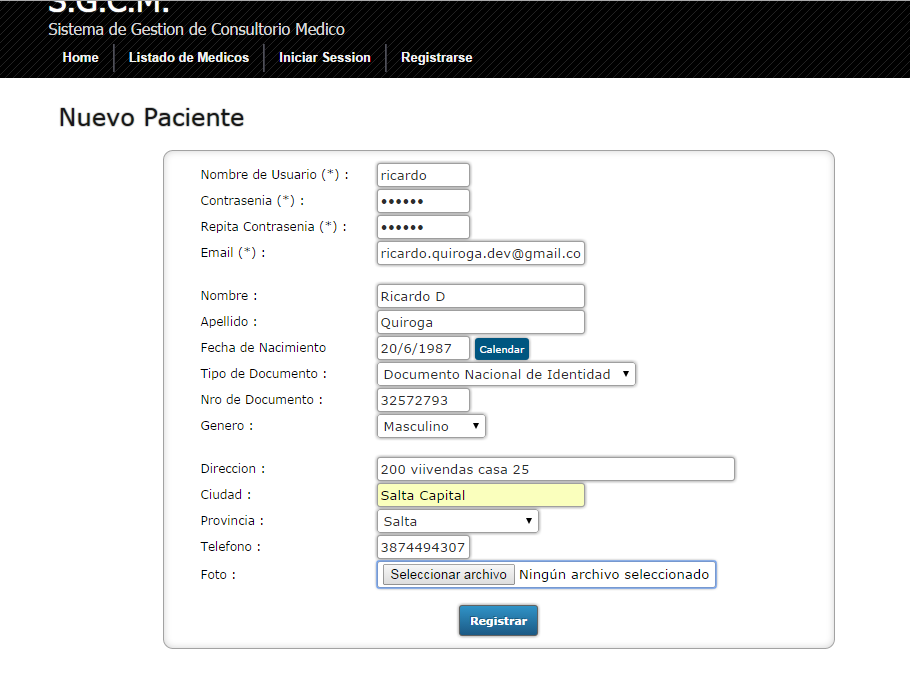
\includegraphics[scale=0.5]{resourse/registrar-paciente.png}
    \caption{Formulario Registro Paciente}
    \label{fig:62}
\end{figure}

Completado el registro y luego de enviado el formulario, si todos los datos son
correctos nos mostrara un mensaje de que el registro fue exitoso:

\begin{figure}[H]
    \centering
    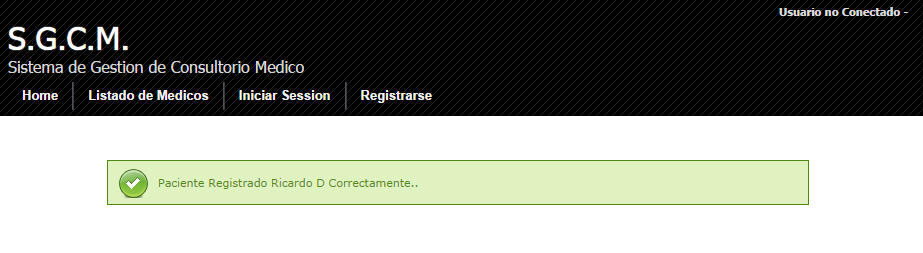
\includegraphics[scale=0.5]{resourse/registro-exito.png}
    \caption{Formulario Registro Paciente}
    \label{fig:63}
\end{figure}

Paso siguiente deveremos revisar nuestra casilla de correo donde nos aparecera
el mensaje con la direccion del formulario para activacion de usuario.
\footnote{Si se intenta iniciar session sin haber activado el usuario nos devolvera
un mensaje de error.}.

\begin{figure}[H]
    \centering
    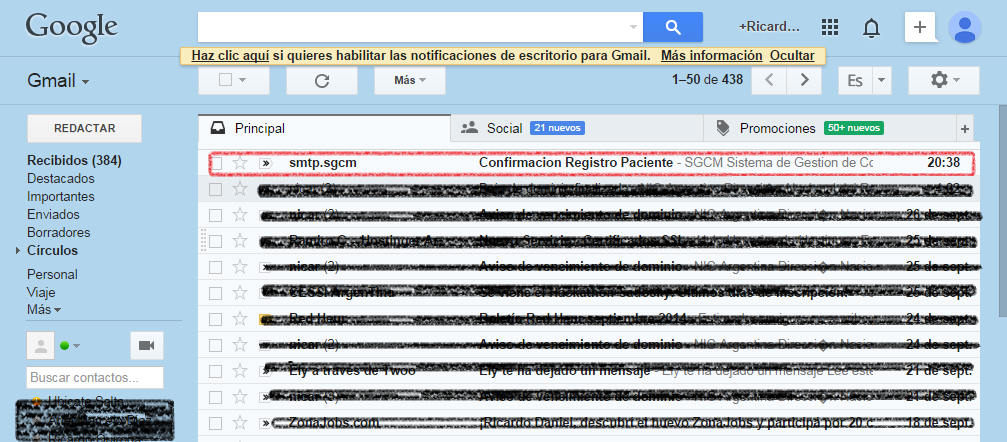
\includegraphics[scale=0.5]{resourse/correo-bandeja.png}
    \caption{Bandeja de Correo con el mensaje}
    \label{fig:64}
\end{figure}

\begin{figure}[H]
    \centering
    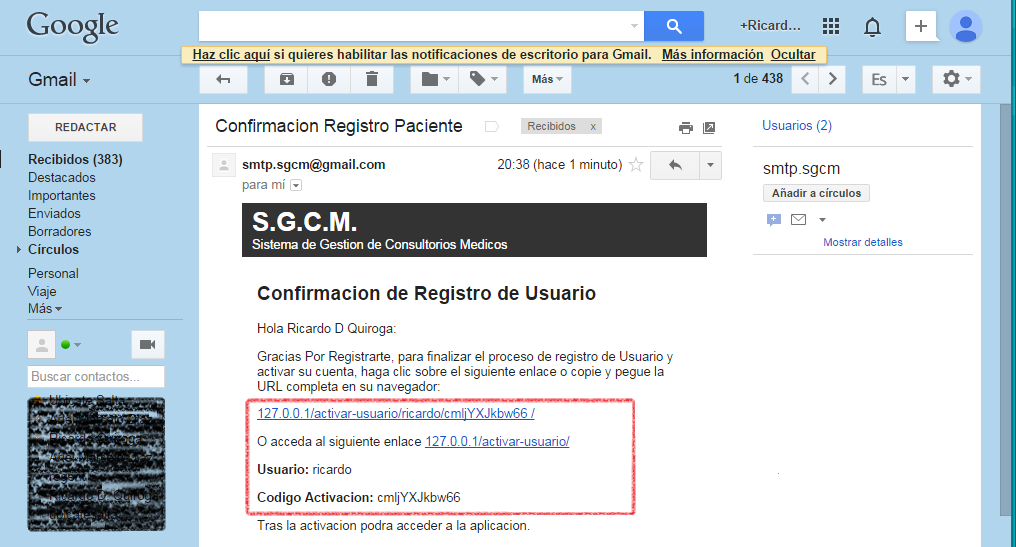
\includegraphics[scale=0.5]{resourse/correo-mensaje.png}
    \caption{Cuerpo del mensaje con la informacion de activacion de usuario}
    \label{fig:65}
\end{figure}

\begin{figure}[H]
    \centering
    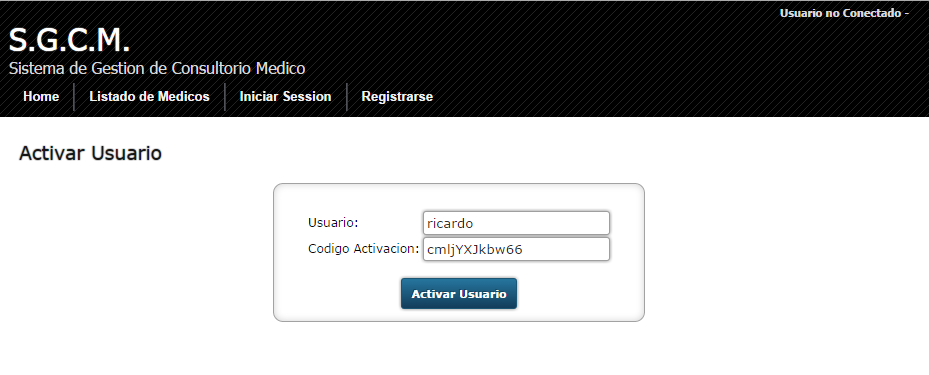
\includegraphics[scale=0.5]{resourse/usuario-activar.png}
    \caption{Formulario de Activacion de usuario}
    \label{fig:66}
\end{figure}

Luego de estos pasos el usuario estara registrado y activado, solo faltaria
iniciar session para poder empezar a operar como paciente.

\subsection{Iniciar Session}

La vista de inicio de session no es nada de otro mundo, solo es un simple
formulario donde debes introducir el usuario y contraseña validos para poder
iniciar session.


\section{Panel de Usuario Paciente}

Corresponde al panel de funciones al que tendran acceso los usuarios, pacientes
sigue siendo limitado pero ya se pueden hacer algunas cosas como solicitar
turnos y realizar consultas medicas rapidas a un expecialista, se organiza en:

\begin{itemize}
    \item \textbf{Inicio}: Ir a la pantalla de Inicio
    \item \textbf{Listado de Medicos}: Mostrar informacion  acerca de los expecialistas.
    \item \textbf{Mensajes}: Casilla de Mensajes Internos.
    \item \textbf{Mis Turnos}: Informacion acerca del estado de los turnos del usuario.
    \item \textbf{Opciones}: Panel de Opciones
\end{itemize}


\subsection{Listado de Medicos}

Vista que permite seleccionar entre el listado de expecialistas que componen el
cuerpo medico de la intitucion consultar informacion, realizar una consulta rapidas
y solicitar turno.

\begin{figure}[H]
    \centering
    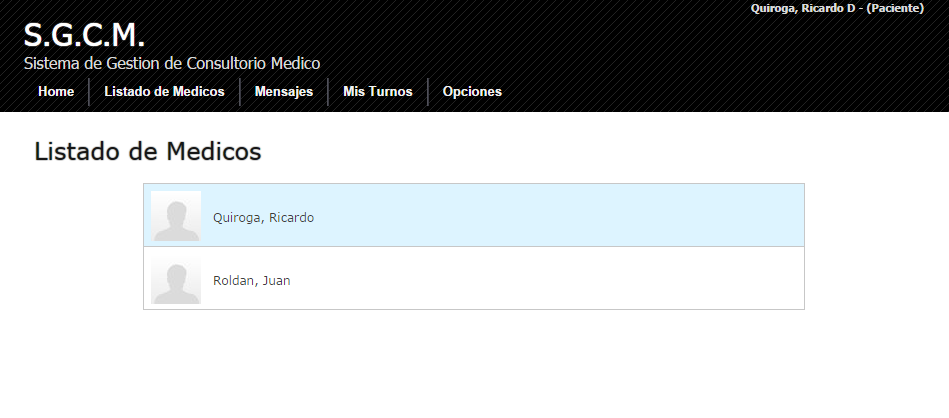
\includegraphics[scale=0.5]{resourse/listado-medico.png}
    \caption{Listado de Medicos}
    \label{fig:67}
\end{figure}

\begin{figure}[H]
    \centering
    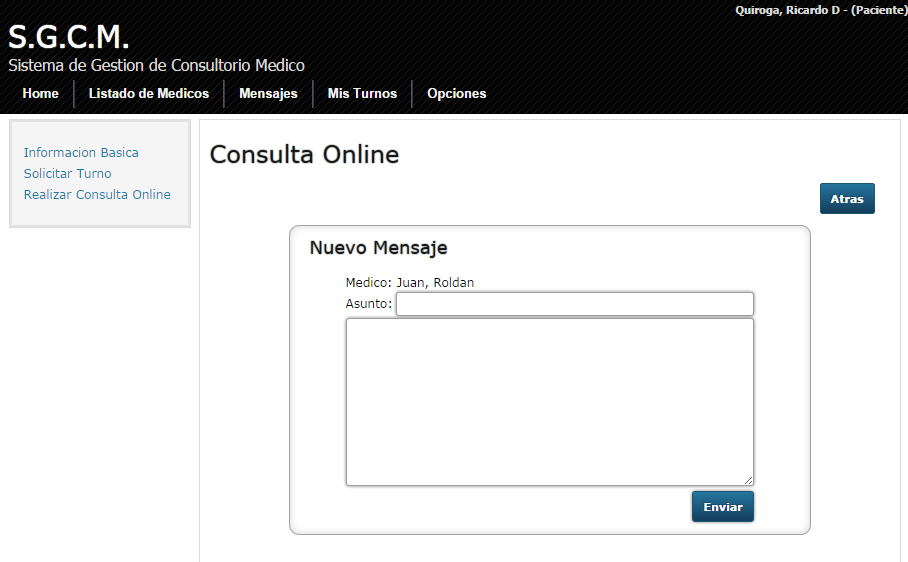
\includegraphics[scale=0.5]{resourse/consulta-online.png}
    \caption{Formulario de Consulta Online}
    \label{fig:68}
\end{figure}

\begin{figure}[H]
    \centering
    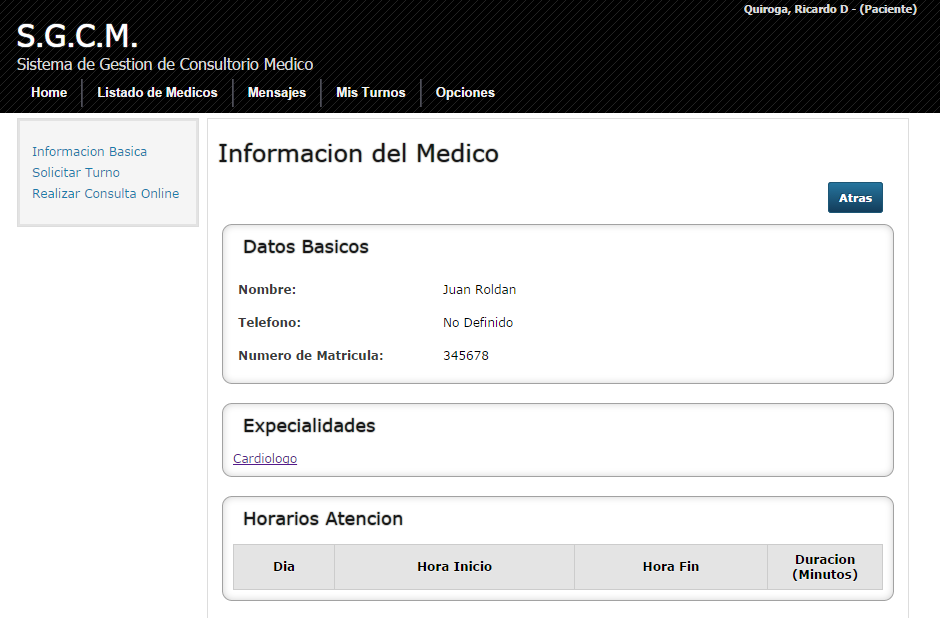
\includegraphics[scale=0.5]{resourse/medico-mostrar.png}
    \caption{Mostrar Datos del Medico}
    \label{fig:69}
\end{figure}

La vista de Asignacion de turno son similares, entre si no varian mucho por lo que
se explicara en la parte del panel de Medico.


\subsection{Mensajes}

Como ya se menciono esto es una session comun a todas los usuarios, se trata de un
conjunto de vista donde funciona el sistema de mensajeria interna entre los usuarios
de la aplicacion, su funcion esta reducida en cuanto al usuario paciente ya que
este solo puede visualizar y responder los mensajes que se le envian, para enviar
un mensaje a un profecional se realiza mediante la opcion de Realizar Consulta
Online, por lo que solo puede enviar mensaje a los expecialistas, las Opciones
disponible son:

\begin{itemize}
    \item \textbf{Redactar}: Escribir un Nuevo Mensaje
    \item \textbf{Recibidos}: Bandeja de Entrada
    \item \textbf{Enviado}: Bandeja de Salida
\end{itemize}

Algunas de las cuales pueden ser apreciadas en las siguientes capturas:

\begin{figure}[H]
    \centering
    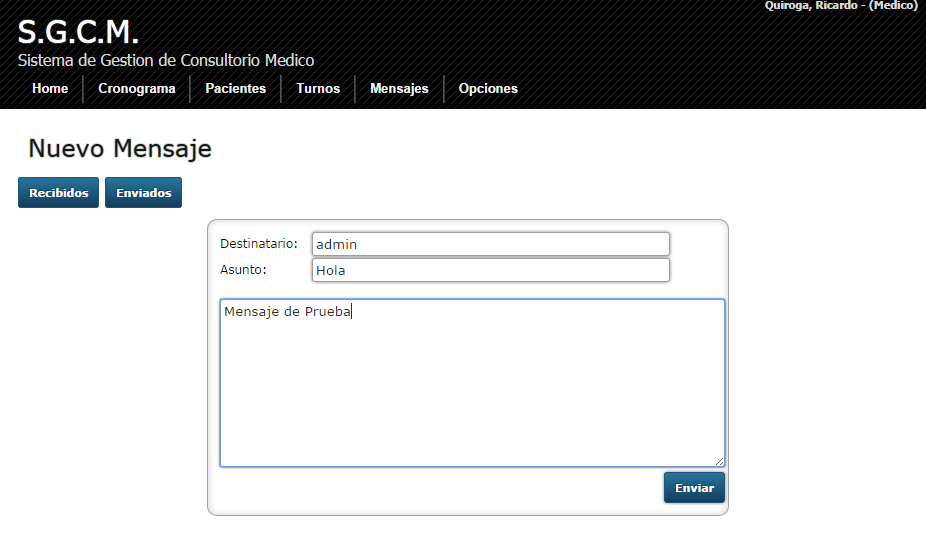
\includegraphics[scale=0.5]{resourse/mensaje-redactar.png}
    \caption{Redactar un Mensaje}
    \label{fig:610}
\end{figure}

\begin{figure}[H]
    \centering
    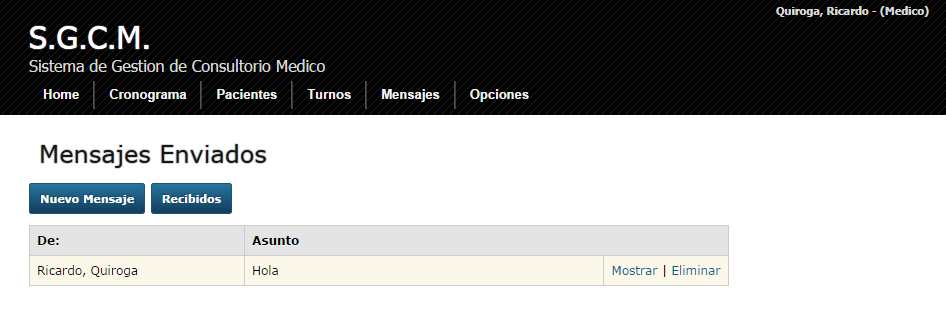
\includegraphics[scale=0.5]{resourse/mensaje-recibidos.png}
    \caption{Bandeja de Entrada}
    \label{fig:611}
\end{figure}

\begin{figure}[H]
    \centering
    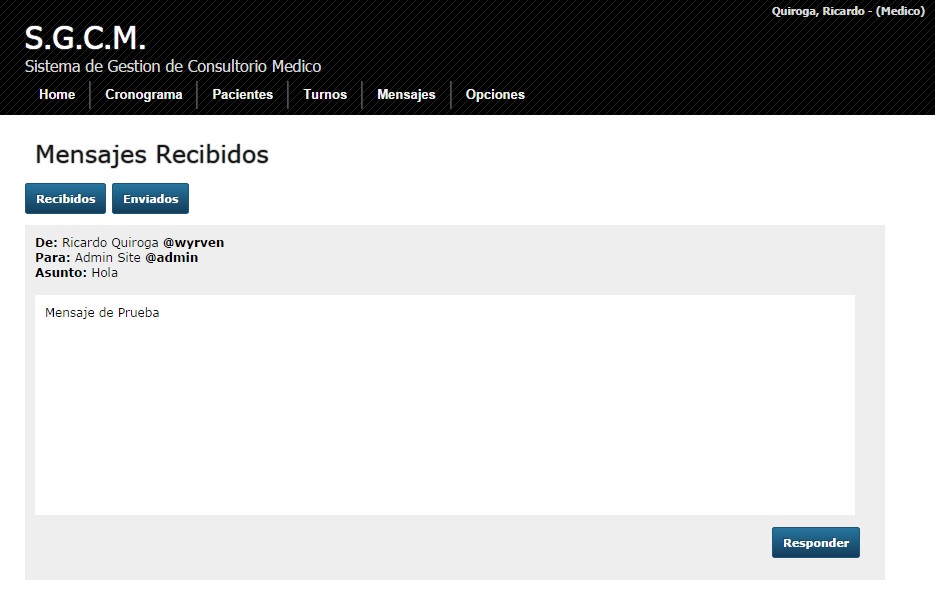
\includegraphics[scale=0.5]{resourse/mensaje-mostrar.png}
    \caption{Mostrar Mensaje}
    \label{fig:612}
\end{figure}

\subsection{Opciones}
Otro menu comun a todo los usuarios permite la administracion de los datos e
informacion del mismo, dentro de las funciones que permite este menu se encuentra:

\begin{itemize}
    \item \textbf{Mis Datos}: Mostrar/Modificar Datos personales
    \item \textbf{Camibar Contrase\~na}: Formulario para cambio de Contrase\~na
    \item \textbf{Cerrar Session}: Cerrar Session, despedirse del sistema.
\end{itemize}


\section{Panel de Usuario Administrativo}

Corresponde al panel de funciones al que tendran acceso los usuarios
Administrativos 

\begin{itemize}
    \item \textbf{Inicio}: Ir a la pantalla de Inicio
    \item \textbf{Pacientes}: Administrar Usuarios Pacientes
    \item \textbf{Medicos}: Administrar Usuarios Medicos
    \item \textbf{Administrativos}: Administrar Usuarios Administrativos
    \item \textbf{Expecialidades}: Administrar Expecialidades Medicas
    \item \textbf{Mensajes}: Casilla de Mensajes Internos.
    \item \textbf{Opciones}: Panel de Opciones
\end{itemize}


\subsection{Pacientes, Medicos, Administrativos}

Los tres conjuntos de vistas comparten muchas caracteristicas similares por lo
que se explican en conjunto y solo se mencionaran algunas de sus diferencias,
cada sub menu se enlista de acuerdo a los tipos de usuarios que se desea
administrar, permitiendo segun el sub menu la posibilidad de crear un tipo de
usuario especifico \footnote{Los Usuarios registrados por el Administrador o el
Medico no requieren activacion como los usuarios creados por usuarios no
registrados.} Buscar un usuario, modifar sus datos.


\begin{figure}[H]
    \centering
    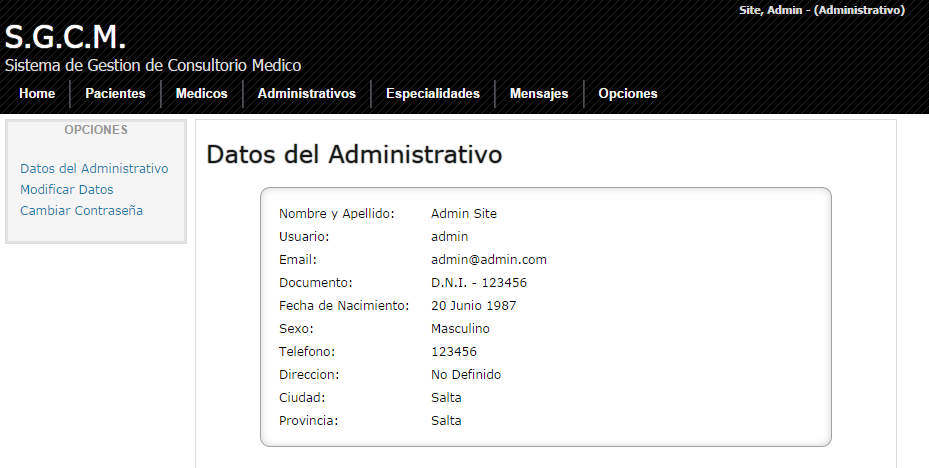
\includegraphics[scale=0.5]{resourse/datos-admin.png}
    \caption{Mostrar Administrativo}
    \label{fig:615}
\end{figure}

\begin{figure}[H]
    \centering
    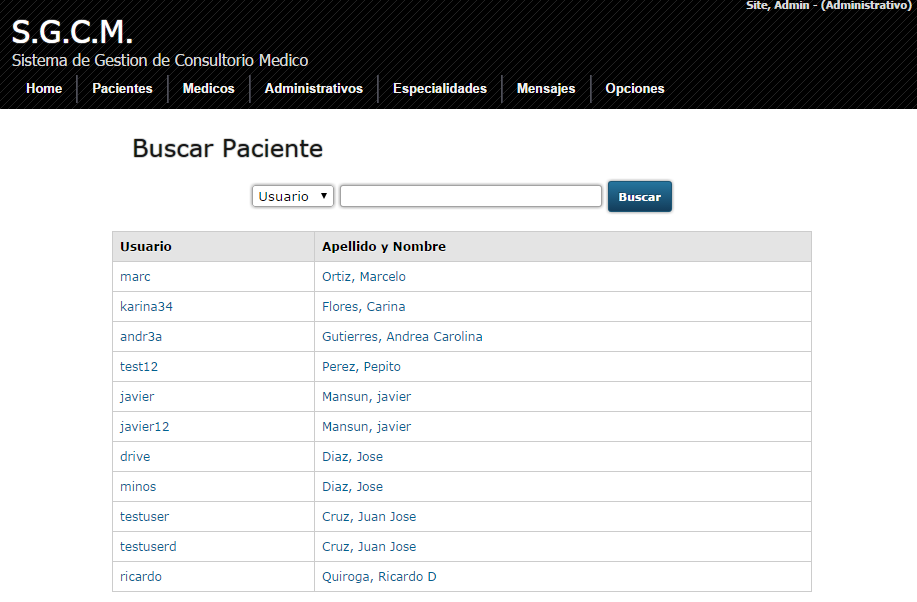
\includegraphics[scale=0.5]{resourse/listado-paciente.png}
    \caption{Vista para busqueda de usuario, en este caso usuarios Pacientes}
    \label{fig:616}
\end{figure}

En el caso de los usuarios medicos ademas puede consultar y modificar el estado
de los turnos que les fueron solicitados, definirles expecialidades
correspondiente.

\begin{figure}[H]
    \centering
    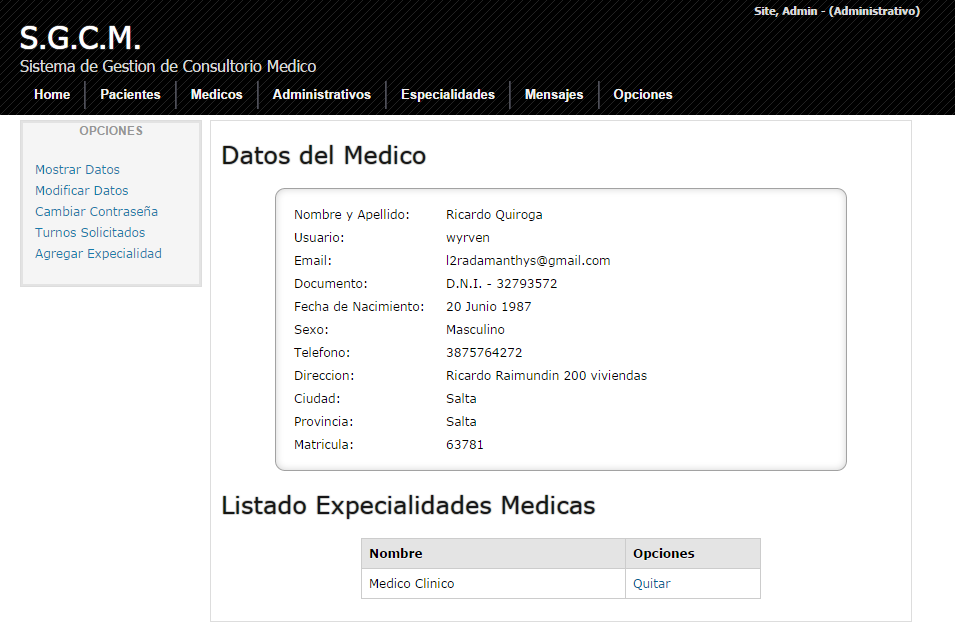
\includegraphics[scale=0.5]{resourse/datos-medico-a.png}
    \caption{Mostrar Medico}
    \label{fig:614}
\end{figure}


\begin{figure}[H]
    \centering
    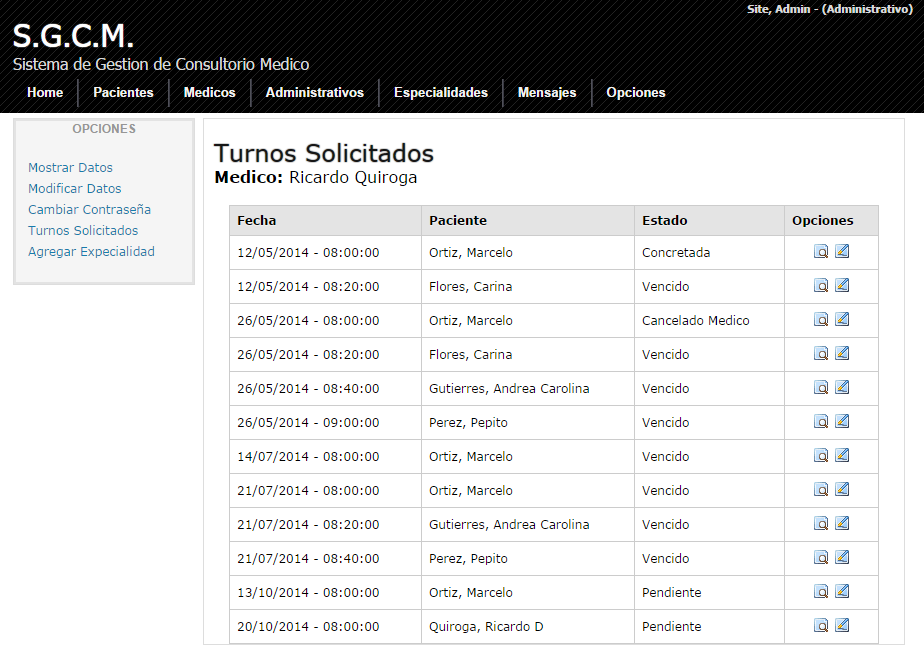
\includegraphics[scale=0.5]{resourse/turnos-sol-medico.png}
    \caption{Vista Listado Turnos Solicitados al Medico.}
    \label{fig:617}
\end{figure}


En los pacientes ademas puede asignar un turno a los mismo, cancelar un turno
solicitado por el mismo, mostrar informacion e impribir comprobante
correspondiente.

\begin{figure}[H]
    \centering
    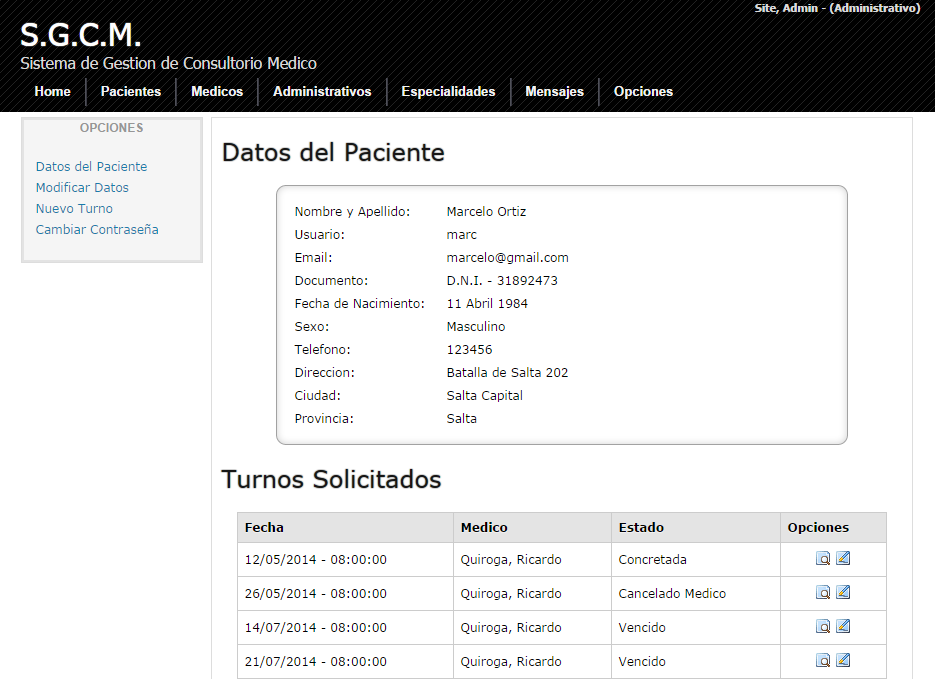
\includegraphics[scale=0.5]{resourse/datos-paciente-a.png}
    \caption{Mostrar Paciente}
    \label{fig:613}
\end{figure}



\section{Panel de Usuario Medicos}

Corresponde al panel de funciones al que tendran acceso los usuarios ...

\begin{itemize}
    \item \textbf{Inicio}: Ir a la pantalla de Inicio
    \item \textbf{Cronograma}:
    \item \textbf{Pacientes}:
    \item \textbf{Turnos}: 
    \item \textbf{Mensajes}: Casilla de Mensajes Internos.
    \item \textbf{Opciones}: Panel de Opciones
\end{itemize}
